% Created by tikzDevice version 0.7.0 on 2014-12-19 12:18:48
% !TEX encoding = UTF-8 Unicode
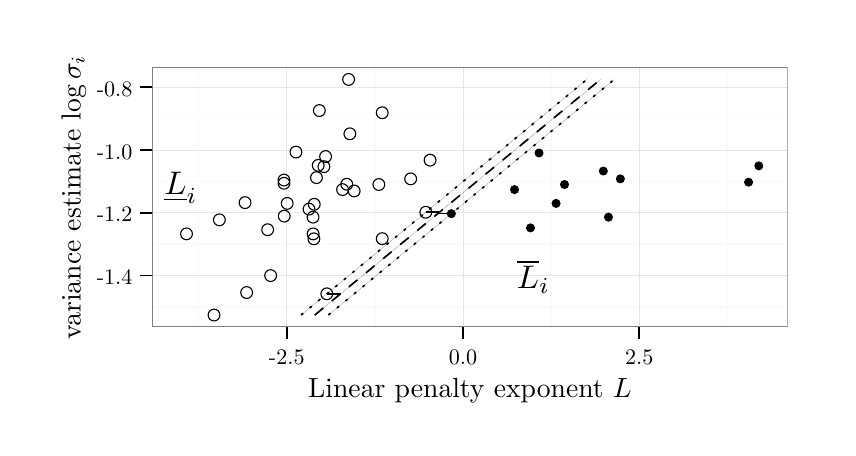
\begin{tikzpicture}[x=1pt,y=1pt]
\definecolor[named]{fillColor}{rgb}{1.00,1.00,1.00}
\path[use as bounding box,fill=fillColor,fill opacity=0.00] (0,0) rectangle (289.08,144.54);
\begin{scope}
\path[clip] (  0.00,  0.00) rectangle (289.08,144.54);
\definecolor[named]{drawColor}{rgb}{1.00,1.00,1.00}
\definecolor[named]{fillColor}{rgb}{1.00,1.00,1.00}

\path[draw=drawColor,line width= 0.6pt,line join=round,line cap=round,fill=fillColor] (  0.00,  0.00) rectangle (289.08,144.54);
\end{scope}
\begin{scope}
\path[clip] ( 44.97, 36.44) rectangle (274.63,130.09);
\definecolor[named]{fillColor}{rgb}{1.00,1.00,1.00}

\path[fill=fillColor] ( 44.97, 36.44) rectangle (274.63,130.09);
\definecolor[named]{drawColor}{rgb}{0.98,0.98,0.98}

\path[draw=drawColor,line width= 0.6pt,line join=round] ( 44.97, 43.71) --
	(274.63, 43.71);

\path[draw=drawColor,line width= 0.6pt,line join=round] ( 44.97, 66.36) --
	(274.63, 66.36);

\path[draw=drawColor,line width= 0.6pt,line join=round] ( 44.97, 89.01) --
	(274.63, 89.01);

\path[draw=drawColor,line width= 0.6pt,line join=round] ( 44.97,111.66) --
	(274.63,111.66);

\path[draw=drawColor,line width= 0.6pt,line join=round] ( 61.78, 36.44) --
	( 61.78,130.09);

\path[draw=drawColor,line width= 0.6pt,line join=round] (125.46, 36.44) --
	(125.46,130.09);

\path[draw=drawColor,line width= 0.6pt,line join=round] (189.15, 36.44) --
	(189.15,130.09);

\path[draw=drawColor,line width= 0.6pt,line join=round] (252.83, 36.44) --
	(252.83,130.09);
\definecolor[named]{drawColor}{rgb}{0.90,0.90,0.90}

\path[draw=drawColor,line width= 0.2pt,line join=round] ( 44.97, 55.03) --
	(274.63, 55.03);

\path[draw=drawColor,line width= 0.2pt,line join=round] ( 44.97, 77.68) --
	(274.63, 77.68);

\path[draw=drawColor,line width= 0.2pt,line join=round] ( 44.97,100.34) --
	(274.63,100.34);

\path[draw=drawColor,line width= 0.2pt,line join=round] ( 44.97,122.99) --
	(274.63,122.99);

\path[draw=drawColor,line width= 0.2pt,line join=round] ( 93.62, 36.44) --
	( 93.62,130.09);

\path[draw=drawColor,line width= 0.2pt,line join=round] (157.31, 36.44) --
	(157.31,130.09);

\path[draw=drawColor,line width= 0.2pt,line join=round] (220.99, 36.44) --
	(220.99,130.09);
\definecolor[named]{drawColor}{rgb}{0.00,0.00,0.00}

\node[text=drawColor,anchor=base,inner sep=0pt, outer sep=0pt, scale=  1.18] at ( 55.41, 84.13) {$\underline L_i$};

\node[text=drawColor,anchor=base,inner sep=0pt, outer sep=0pt, scale=  1.18] at (182.78, 50.15) {$\overline L_i$};

\path[draw=drawColor,line width= 0.4pt,line join=round,line cap=round] (143.86, 77.84) circle (  2.13);

\path[draw=drawColor,line width= 0.4pt,line join=round,line cap=round] (145.41, 96.66) circle (  2.13);

\path[draw=drawColor,line width= 0.4pt,line join=round,line cap=round] (103.15, 70.02) circle (  2.13);

\path[draw=drawColor,line width= 0.4pt,line join=round,line cap=round] ( 86.72, 71.53) circle (  2.13);

\path[draw=drawColor,line width= 0.4pt,line join=round,line cap=round] (104.35, 90.35) circle (  2.13);

\path[draw=drawColor,line width= 0.4pt,line join=round,line cap=round] ( 57.39, 70.03) circle (  2.13);

\path[draw=drawColor,line width= 0.4pt,line join=round,line cap=round] (107.65, 97.98) circle (  2.13);

\path[draw=drawColor,line width= 0.4pt,line join=round,line cap=round] (103.12, 76.07) circle (  2.13);

\path[draw=drawColor,line width= 0.4pt,line join=round,line cap=round] (117.98, 85.53) circle (  2.13);

\path[draw=drawColor,line width= 0.4pt,line join=round,line cap=round] ( 67.34, 40.70) circle (  2.13);

\path[draw=drawColor,line width= 0.4pt,line join=round,line cap=round] (108.10, 48.37) circle (  2.13);

\path[draw=drawColor,line width= 0.4pt,line join=round,line cap=round] (101.66, 78.97) circle (  2.13);

\path[draw=drawColor,line width= 0.4pt,line join=round,line cap=round] (105.39,114.59) circle (  2.13);

\path[draw=drawColor,line width= 0.4pt,line join=round,line cap=round] (128.12,113.80) circle (  2.13);

\path[draw=drawColor,line width= 0.4pt,line join=round,line cap=round] (138.39, 89.91) circle (  2.13);

\path[draw=drawColor,line width= 0.4pt,line join=round,line cap=round] ( 92.61, 89.46) circle (  2.13);

\path[draw=drawColor,line width= 0.4pt,line join=round,line cap=round] ( 96.95, 99.59) circle (  2.13);

\path[draw=drawColor,line width= 0.4pt,line join=round,line cap=round] ( 87.79, 54.95) circle (  2.13);

\path[draw=drawColor,line width= 0.4pt,line join=round,line cap=round] (113.78, 86.03) circle (  2.13);

\path[draw=drawColor,line width= 0.4pt,line join=round,line cap=round] (116.42,106.19) circle (  2.13);

\path[draw=drawColor,line width= 0.4pt,line join=round,line cap=round] ( 78.55, 81.32) circle (  2.13);

\path[draw=drawColor,line width= 0.4pt,line join=round,line cap=round] (115.30, 87.97) circle (  2.13);

\path[draw=drawColor,line width= 0.4pt,line join=round,line cap=round] ( 93.78, 81.04) circle (  2.13);

\path[draw=drawColor,line width= 0.4pt,line join=round,line cap=round] (104.98, 94.77) circle (  2.13);

\path[draw=drawColor,line width= 0.4pt,line join=round,line cap=round] ( 69.27, 75.10) circle (  2.13);

\path[draw=drawColor,line width= 0.4pt,line join=round,line cap=round] (103.43, 68.24) circle (  2.13);

\path[draw=drawColor,line width= 0.4pt,line join=round,line cap=round] (128.11, 68.30) circle (  2.13);

\path[draw=drawColor,line width= 0.4pt,line join=round,line cap=round] ( 79.12, 48.83) circle (  2.13);

\path[draw=drawColor,line width= 0.4pt,line join=round,line cap=round] (103.55, 80.72) circle (  2.13);

\path[draw=drawColor,line width= 0.4pt,line join=round,line cap=round] ( 92.71, 76.44) circle (  2.13);

\path[draw=drawColor,line width= 0.4pt,line join=round,line cap=round] (126.89, 87.87) circle (  2.13);

\path[draw=drawColor,line width= 0.4pt,line join=round,line cap=round] (115.96,125.83) circle (  2.13);

\path[draw=drawColor,line width= 0.4pt,line join=round,line cap=round] ( 92.63, 88.31) circle (  2.13);

\path[draw=drawColor,line width= 0.4pt,line join=round,line cap=round] (107.04, 94.32) circle (  2.13);
\definecolor[named]{fillColor}{rgb}{0.00,0.00,0.00}

\path[draw=drawColor,line width= 0.4pt,line join=round,line cap=round,fill=fillColor] (184.78, 99.26) circle (  1.42);

\path[draw=drawColor,line width= 0.4pt,line join=round,line cap=round,fill=fillColor] (260.49, 88.70) circle (  1.42);

\path[draw=drawColor,line width= 0.4pt,line join=round,line cap=round,fill=fillColor] (181.68, 72.19) circle (  1.42);

\path[draw=drawColor,line width= 0.4pt,line join=round,line cap=round,fill=fillColor] (209.87, 76.07) circle (  1.42);

\path[draw=drawColor,line width= 0.4pt,line join=round,line cap=round,fill=fillColor] (264.19, 94.61) circle (  1.42);

\path[draw=drawColor,line width= 0.4pt,line join=round,line cap=round,fill=fillColor] (214.17, 89.91) circle (  1.42);

\path[draw=drawColor,line width= 0.4pt,line join=round,line cap=round,fill=fillColor] (175.92, 86.03) circle (  1.42);

\path[draw=drawColor,line width= 0.4pt,line join=round,line cap=round,fill=fillColor] (190.94, 81.04) circle (  1.42);

\path[draw=drawColor,line width= 0.4pt,line join=round,line cap=round,fill=fillColor] (208.01, 92.73) circle (  1.42);

\path[draw=drawColor,line width= 0.4pt,line join=round,line cap=round,fill=fillColor] (153.10, 77.33) circle (  1.42);

\path[draw=drawColor,line width= 0.4pt,line join=round,line cap=round,fill=fillColor] (193.98, 87.87) circle (  1.42);

\path[draw=drawColor,line width= 0.6pt,dash pattern=on 4pt off 4pt ,line join=round,fill=fillColor] (103.74, 40.70) -- (207.00,125.83);

\path[draw=drawColor,line width= 0.6pt,dash pattern=on 1pt off 3pt ,line join=round,fill=fillColor] (108.67, 40.70) -- (211.94,125.83);

\path[draw=drawColor,line width= 0.6pt,dash pattern=on 1pt off 3pt ,line join=round,fill=fillColor] ( 98.80, 40.70) -- (202.07,125.83);

\path[draw=drawColor,line width= 0.6pt,line join=round,fill=fillColor] (143.86, 77.84) -- (148.79, 77.84);

\path[draw=drawColor,line width= 0.6pt,line join=round,fill=fillColor] (108.10, 48.37) -- (113.04, 48.37);

\path[draw=drawColor,line width= 0.6pt,line join=round,fill=fillColor] (153.10, 77.33) -- (148.17, 77.33);
\definecolor[named]{drawColor}{rgb}{0.50,0.50,0.50}

\path[draw=drawColor,line width= 0.6pt,line join=round,line cap=round] ( 44.97, 36.44) rectangle (274.63,130.09);
\end{scope}
\begin{scope}
\path[clip] (  0.00,  0.00) rectangle (289.08,144.54);
\definecolor[named]{drawColor}{rgb}{0.00,0.00,0.00}

\node[text=drawColor,anchor=base east,inner sep=0pt, outer sep=0pt, scale=  0.80] at ( 37.86, 51.73) {-1.4};

\node[text=drawColor,anchor=base east,inner sep=0pt, outer sep=0pt, scale=  0.80] at ( 37.86, 74.38) {-1.2};

\node[text=drawColor,anchor=base east,inner sep=0pt, outer sep=0pt, scale=  0.80] at ( 37.86, 97.03) {-1.0};

\node[text=drawColor,anchor=base east,inner sep=0pt, outer sep=0pt, scale=  0.80] at ( 37.86,119.68) {-0.8};
\end{scope}
\begin{scope}
\path[clip] (  0.00,  0.00) rectangle (289.08,144.54);
\definecolor[named]{drawColor}{rgb}{0.00,0.00,0.00}

\path[draw=drawColor,line width= 0.6pt,line join=round] ( 40.70, 55.03) --
	( 44.97, 55.03);

\path[draw=drawColor,line width= 0.6pt,line join=round] ( 40.70, 77.68) --
	( 44.97, 77.68);

\path[draw=drawColor,line width= 0.6pt,line join=round] ( 40.70,100.34) --
	( 44.97,100.34);

\path[draw=drawColor,line width= 0.6pt,line join=round] ( 40.70,122.99) --
	( 44.97,122.99);
\end{scope}
\begin{scope}
\path[clip] (  0.00,  0.00) rectangle (289.08,144.54);
\definecolor[named]{drawColor}{rgb}{0.00,0.00,0.00}

\path[draw=drawColor,line width= 0.6pt,line join=round] ( 93.62, 32.18) --
	( 93.62, 36.44);

\path[draw=drawColor,line width= 0.6pt,line join=round] (157.31, 32.18) --
	(157.31, 36.44);

\path[draw=drawColor,line width= 0.6pt,line join=round] (220.99, 32.18) --
	(220.99, 36.44);
\end{scope}
\begin{scope}
\path[clip] (  0.00,  0.00) rectangle (289.08,144.54);
\definecolor[named]{drawColor}{rgb}{0.00,0.00,0.00}

\node[text=drawColor,anchor=base,inner sep=0pt, outer sep=0pt, scale=  0.80] at ( 93.62, 22.72) {-2.5};

\node[text=drawColor,anchor=base,inner sep=0pt, outer sep=0pt, scale=  0.80] at (157.31, 22.72) {0.0};

\node[text=drawColor,anchor=base,inner sep=0pt, outer sep=0pt, scale=  0.80] at (220.99, 22.72) {2.5};
\end{scope}
\begin{scope}
\path[clip] (  0.00,  0.00) rectangle (289.08,144.54);
\definecolor[named]{drawColor}{rgb}{0.00,0.00,0.00}

\node[text=drawColor,anchor=base,inner sep=0pt, outer sep=0pt, scale=  1.00] at (159.80, 10.84) {Linear penalty exponent $L$};
\end{scope}
\begin{scope}
\path[clip] (  0.00,  0.00) rectangle (289.08,144.54);
\definecolor[named]{drawColor}{rgb}{0.00,0.00,0.00}

\node[text=drawColor,rotate= 90.00,anchor=base,inner sep=0pt, outer sep=0pt, scale=  1.00] at ( 19.11, 83.26) {variance estimate $\log\sigma_i$};
\end{scope}
\end{tikzpicture}
